% This is the Reed College LaTeX thesis template. Most of the work 
% for the document class was done by Sam Noble (SN), as well as this
% template. Later comments etc. by Ben Salzberg (BTS). Additional
% restructuring and APA support by Jess Youngberg (JY).
% Your comments and suggestions are more than welcome; please email
% them to cusf@reed.edu
%
% See http://web.reed.edu/cis/help/latex.html for help. There are a 
% great bunch of help pages there, with notes on
% getting started, bibtex, etc. Go there and read it if you're not
% already familiar with LaTeX.
%
% Any line that starts with a percent symbol is a comment. 
% They won't show up in the document, and are useful for notes 
% to yourself and explaining commands. 
% Commenting also removes a line from the document; 
% very handy for troubleshooting problems. -BTS

% As far as I know, this follows the requirements laid out in 
% the 2002-2003 Senior Handbook. Ask a librarian to check the 
% document before binding. -SN

%%
%% Preamble
%%
% \documentclass{<something>} must begin each LaTeX document
\documentclass[12pt,twoside]{reedthesis}
% Packages are extensions to the basic LaTeX functions. Whatever you
% want to typeset, there is probably a package out there for it.
% Chemistry (chemtex), screenplays, you name it.
% Check out CTAN to see: http://www.ctan.org/
%%
\usepackage{graphicx,latexsym} 
\usepackage{amssymb,amsthm,amsmath}
\usepackage{longtable,booktabs,setspace} 
\usepackage{subfig}
%\usepackage{chemarr} %% Useful for one reaction arrow, useless if you're not a chem major
\usepackage{url}
\usepackage{natbib}
\usepackage{pdfpages}
\usepackage{fancyvrb}
\usepackage{multirow}
% \usepackage{times} % other fonts are available like times, bookman, charter, palatino

\newcommand{\eqn}[1]{\begin{equation}#1\end{equation}}
\newcommand{\eq}[1]{\begin{align}#1\end{align}}
\newcommand{\fig}[2]{\begin{figure}\begin{center}#1\end{center}#2\end{figure}}



\title{Quantum Mechanical Bound States of the Yukawa Potential (or some better title)}
\author{Ellen M. McManis}
% The month and year that you submit your FINAL draft TO THE LIBRARY (May or December)
\date{May 2012}
\division{Mathematics and Natural Sciences}
\advisor{Nelia Mann}
%If you have two advisors for some reason, you can use the following
%\altadvisor{Your Other Advisor}
%%% Remember to use the correct department!
\department{Physics}
% if you're writing a thesis in an interdisciplinary major,
% uncomment the line below and change the text as appropriate.
% check the Senior Handbook if unsure.
%\thedivisionof{The Established Interdisciplinary Committee for}
% if you want the approval page to say "Approved for the Committee",
% uncomment the next line
%\approvedforthe{Committee}

\setlength{\parskip}{0pt}
%%
%% End Preamble
%%
%% The fun begins:
\begin{document}

  \maketitle
  \frontmatter % this stuff will be roman-numbered
  \pagestyle{empty} % this removes page numbers from the frontmatter

% Acknowledgements (Acceptable American spelling) are optional
% So are Acknowledgments (proper English spelling)
    \chapter*{Acknowledgements}
	People. Things. Shep, the dog who is currently keeping me company.

% The preface is optional
% To remove it, comment it out or delete it.
%    \chapter*{Preface}
%	This is an example of a thesis setup to use the reed thesis document class.

    \tableofcontents
% if you want a list of tables, optional
    \listoftables
% if you want a list of figures, also optional
    \listoffigures

% The abstract is not required if you're writing a creative thesis (but aren't they all?)
% If your abstract is longer than a page, there may be a formatting issue.
    \chapter*{Abstract}
	Math and computers and stuff gave me results!
		
%	\chapter*{Dedication}
%	You can have a dedication here if you wish.

  \mainmatter % here the regular arabic numbering starts
  \pagestyle{fancyplain} % turns page numbering back on

%The \introduction command is provided as a convenience.
%if you want special chapter formatting, you'll probably want to avoid using it altogether

    \chapter*{Introduction}
         \addcontentsline{toc}{chapter}{Introduction}
	\chaptermark{Introduction}
	\markboth{Introduction}{Introduction}
	% The three lines above are to make sure that the headers are right, that the intro gets included in the table of contents, and that it doesn't get numbered 1 so that chapter one is 1.

% Double spacing: if you want to double space, or one and a half 
% space, uncomment one of the following lines. You can go back to 
% single spacing with the \singlespacing command.
% \onehalfspacing
% \doublespacing
The Yukawa potential describes a force mediated by a massive particle. It is %argh fuck this part
\eqn{
V(r) = -\frac{C}{r}e^{-r/l}\mbox{,}
}
where $C$ and $l$ are constants. $C$ sets the strength of the force; $l$ acts as a length scale. The exponential term provides an effective cutoff for the associated force once $r$ gets much larger than $l$, as the exponential term drops off quite rapidly. We are interested in how the bound states of a particle subject to this potential change with these constants. 

The length scale of the potential, which limits the range at which the force acts, is related to the mass of the mediating particle $m$ by the equation\eqn{
l = \frac{\hbar}{m c}\mbox{.}
}
Both the mass $m$ and the strength of the force $C$ depend on the application of the potential. Most commonly, we use this potential to describe the force between protons and neutrons in an atomic nucleus, where $m$ is the mass of the pion, $m_{\pi} = 140$ MeV/c$^2$.\footnote{I know I'm missing numbers here, will add}

In general, to find the bound states of a particle under the influence of some $V(r)$, we solve the time-independent Schr\"odinger wave equation
\eqn{
-\frac{\hbar^2}{2\mu}\nabla^2\psi(r,\phi,\theta) + V(r)\psi (r,\phi,\theta) = E \psi(r,\phi,\theta)
\label{eq:TIDSWE-general}
} and look for solutions which go to zero at infinity.
%In this thesis, we are working with a system of two particles attracted to each other by the Yukawa potential. To simplify the system, it makes the most sense to express this in spherical coordinates as a reduced mass orbiting a center of mass. This is the form used by the wave equation above. 
With the Yukawa potential, this equation cannot be solved analytically. However, in the limit where $r >> l$, the exponential term disappears, leaving
\eqn{
V(r) \approx -\frac{C}{r}\mbox{.}
\label{eq:vapprox}
}
This is the same form as the Coulomb potential (in which $C = \frac{e^2}{4\pi\epsilon_0}$), which we use to find the bound states of an electron and a proton in Hydrogen. \eqref{eq:vapprox} suggests that we will be able to gain some insight into the Yukawa potential by looking at the solutions to the wave equation for the Coulomb potential. 

These solutions are:
\eqn{
\psi_{l, m_l, n} (r, \theta, \phi) = R_{n,l}(r) Y_{l,m_l}(\theta,\phi)\mbox{.}
}
Here, $l$, $m_l$, and $n$ are quantum numbers. The $Y_{l, m_l}$ are the spherical harmonics. For simplicity, we begin by focusing on states with zero angular momentum, for which the solutions are spherically symmetric.
For convenience, we introduce a length scale, 
\eqn{
\alpha = \frac{\hbar^2}{C \mu}\mbox{.}
\label{eq:bohrradius}
}
which is a constant with units of length, defined in terms of the other constants of the problem. 
In hydrogen, this is the Bohr radius, and reduces to the familiar $a_o = \frac{4\pi \epsilon_0 \hbar^2}{\mu e^2}$. For deuterium, if we insert the appropriate numbers [...numbers] 
We can now take $Y_{0,0} = 1/\sqrt{4 \pi}$, leaving us with
\eqn{
\psi_{n, l =0}(r) = R_{n , l= 0}(r) = \frac{1}{\sqrt{4\pi}} e^{-r /\alpha n}L_{n-1} \left(2\frac{r}{ \alpha n}\right)
\label{eq:SWE-coulomb}
}
where $L_{n-1}$ is a Laguerre polynomial. 

The factor of $e^{-r /\alpha n}$ ensures that the wave function goes to 0 as $r$ goes to infinity, with $n$ controlling how fast that happens. The Laguerre polynomial determines how many nodes the wave function has. Because $L_{n-1}$ has $n-1$ roots, so the wave function will have that many nodes (figure \ref{fig:wavefunctions}).
\begin{figure}[h]
\centering
\subfloat[]{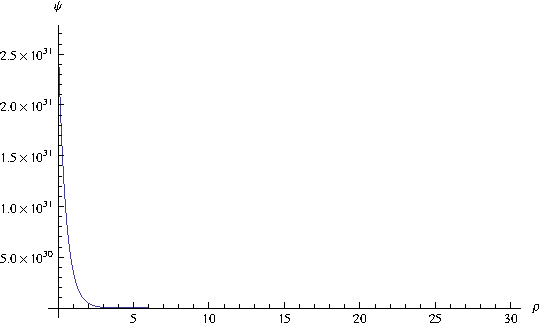
\includegraphics[width=0.3\textwidth]{Figures/ps0}}
\subfloat[]{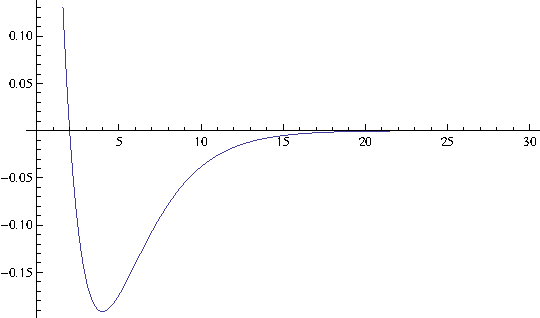
\includegraphics[width=0.3\textwidth]{Figures/ps1}}
\subfloat[]{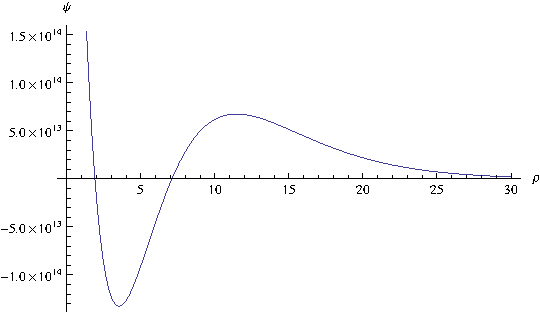
\includegraphics[width=0.3\textwidth]{Figures/ps2}}
\caption{The first three bound states of $\psi(\rho)$ for the Coulomb potential, where $\rho = r/\alpha$. These show the nodes given by the Laguerre polynomials as well as the exponential dieoff of the wave function.}
\label{fig:wavefunctions}
\end{figure}

The energy for the particle described by this wave function is just a function of $n$ (the principal quantum number), and is equal to
\eqn{
E_n = -\frac{C}{2\alpha n^2}\mbox{.}
\label{eq:henergy}
}
There are an infinite number of bound states labelled by n, and as n gets large, the energies given by \eqref{eq:henergy} get closer and closer to zero but never quite reach it (the states remain bound). As this happens, the wave functions can be found further and further from the origin. This effect can be seen in figure \ref{fig:boundstates} in which the first six bound states are plotted.

\begin{figure}[h]
\centering
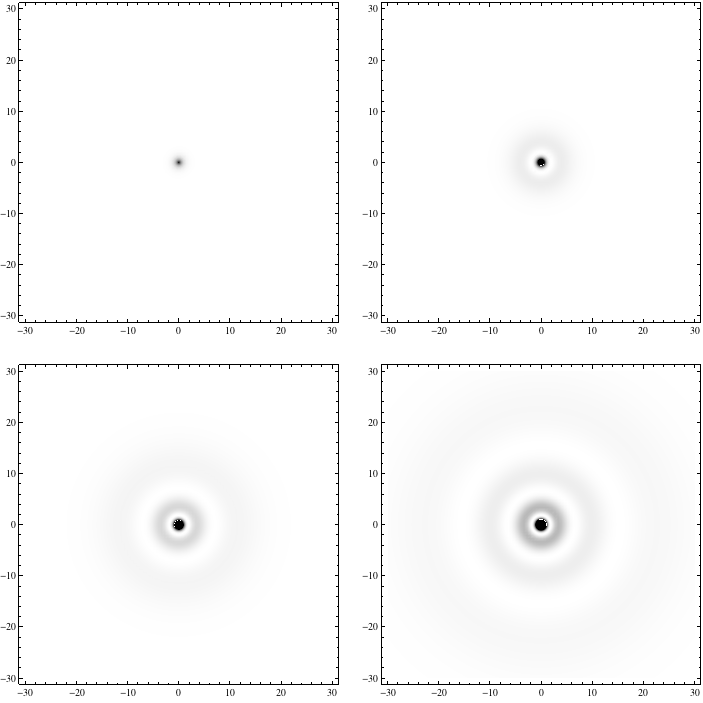
\includegraphics{Figures/densityplots}
\caption[Density plots of the first six spherically symmetric Coulomb wave functions]{The first six spherically symmetric wave functions. This plot shows the probability density, $\psi(\rho)^2$, in spherical coordinates. These plots are all close to the origin, where $\psi$ is large.}
\label{fig:boundstates}
\end{figure}

Now let us consider how this changes for the Yukawa potential, which itself has an exponential die-off with length scale $l$. Because of \eqref{eq:vapprox}, we expect the Yukawa states to resemble the Coulomb states for bound states with $r << l$. For $r >> l$, the potential is approximately $0$. We do not expect to find any bound states where the wave function is significantly non-zero in this region, because there is no force to bind the particle. We therefore expect that the number of bound states of this potential will be be finite.

When working with the Yukawa problem, we will continue using the length scale alpha from \eqref{eq:bohrradius}. What we are interested in is not $l$ itself, but the ratio $l / \alpha$.
If $l / \alpha$ is small, a given state is more likely to fall outside of the range of the potential, meaning that only a small number of states (those whose wave functions do not extend very far out) may be bound. For a large $l / \alpha$, the reverse is true, and we expect a large number of bound states.

%\begin{figure}[h]
%\begin{center}
%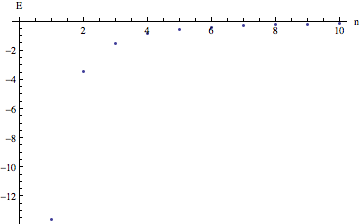
\includegraphics[scale=0.7]{Figures/hydrogenspectrum}
%\end{center}
%\caption{The energies of the first 10 bound states of the electron in the hydrogen atom}
%\label{fig:hspec}
%\end{figure}
\clearpage %% starts a new page and stops trying to place floats such as tables and figures

\chapter{Semi-Classical Approximation}
\section{The Bohr Model}
To better understand the relationship between the number of bound states and $l$, we begin with a semi-clasical approximation. This will give us an idea what to expect from the numerical analysis. For this approximation we can again exploit the similarities between the Yukawa potential when $r << l$ and the Coulomb potential and use the Bohr model. 
%The Bohr model is most commonly applied to the electron orbiting the nucleus in hydrogen. 
The postulates of the model include the following:
\begin{enumerate}
\item Particles move in circular orbits around the center under the influence of some potential $V(r)$. They obey all the laws of classical mechanics.
\item Angular momentum is quantized; $L = n\hbar$ where $n$ is a positive integer.
\end{enumerate}

To use these postulates, first, we look at the classical energy of a particle moving under the influence of the potential:
\eqn{
E = \frac{1}{2}\mu \dot{r}^2+\frac{1}{2}\frac{(n \hbar)^2}{\mu r^2}-V(r)\mbox{.}
\label{eq:classical-energy}
}

We can roll the second half of the equation up into an effective potential, producing something of the form $E = KE + PE$. The effective potential $V_{\mathrm{eff}}$ is then
\eqn{
V_{\mathrm{eff}}(r)=\frac{(n \hbar)^2}{2 \mu}\frac{1}{r^2}+V(r)
\label{eq:veff}
}
Referring back to the first postulate, we know that our semi-classical particle is moving in a circular orbit. Classically, a circular orbit occurs when the effective potential is minimized, that is, when
\eqn{
\frac{dV_{\mathrm{eff}}}{d r}\Big |_{r = r_0}= 0
\label{eq:vrnaught}
}
Given some $n$, the radius of the Bohr orbit will be given by \eqref{eq:vrnaught}. The energy of this orbit will be given by evaluating \eqref{eq:classical-energy}
 at $r_0$. Because the orbit is circular, $\dot{r} = 0$, so the energy will be given by
\eqn{
E_{n} = \frac{1}{2}\frac{(n\hbar)^2}{\mu r_0^2} - V(r_0)\mbox{.}
}

\section{Application to Coulomb potential}
Let's remind ourselves how this works for the Coulomb potential. To make this easier to work with, we use the length scale from \eqref{eq:bohrradius}, the ``Bohr radius'' for this problem. We then use this to nondimensionalize $r$, defining
\begin{equation}
\rho \equiv \frac{r}{\alpha}\mbox{.}
\label{eq:rho}
\end{equation}
We also define a time scale:
\begin{equation}
\beta \equiv \frac{C^2m}{\hbar^3}\mbox{.}
\label{eq:beta}
\end{equation}
We can substitute these into \eqref{eq:classical-energy} and \eqref{eq:veff} in order to obtain nondimensionalize:
\eqn{
\frac{2 \alpha}{C}E = \tilde{E}= \rho '^2 + \frac{n^2}{\rho^2}-\frac{2}{\rho}
\label{eq:energy-nondim}
}
\eqn{
\tilde{V}_{\mathrm{eff}} = \frac{n^2}{\rho^2}-\frac{2}{\rho}
\label{eq:veff-nondim}
}

We can plot the effective potential vs $\rho$ (figure \ref{fig:hveff}). The circular orbits will be at the minimum of this effective potential, where the radius of the particle's orbit is constant. Note that a different value of $n$ gives a different effective potential with a different minimum. 

\begin{figure}[h]
\center{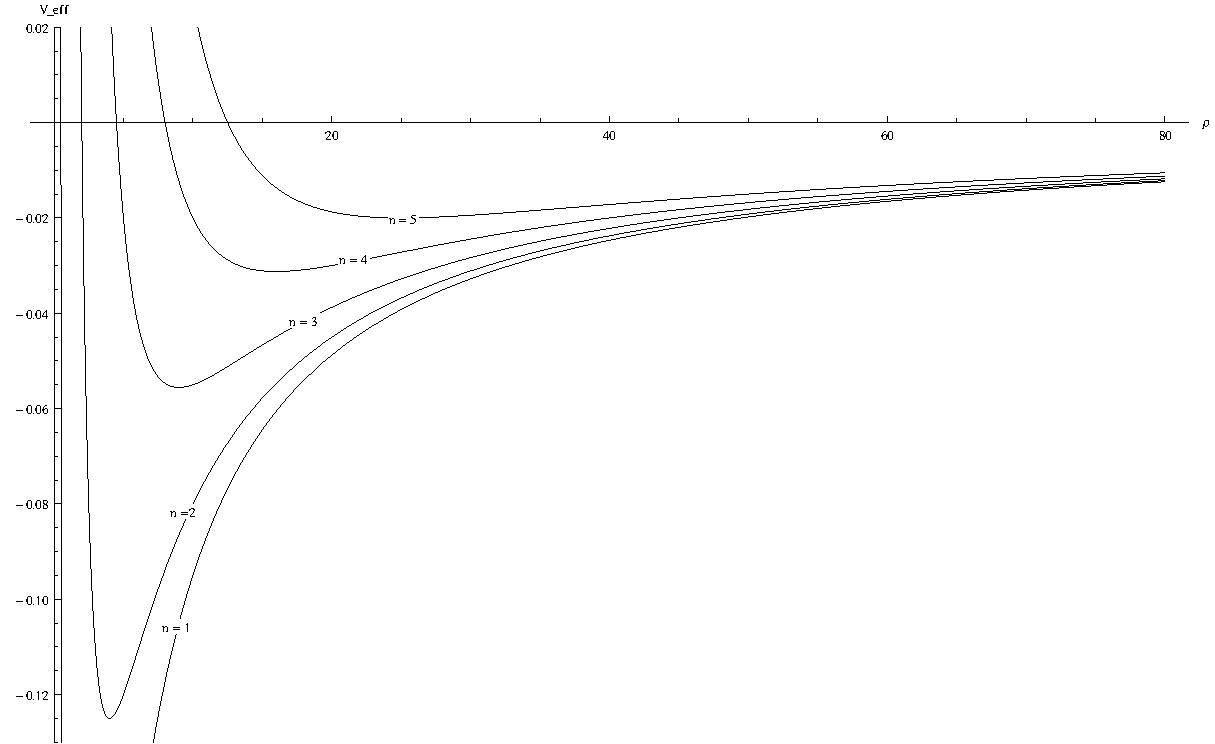
\includegraphics[width=\textwidth]{Figures/hyd_Veff}}
\caption{The effective Coulomb potential. Particles can exist with energies greater than the potential energy, and their trajectories will cover all possible radii at that energy. A particle in a circular orbit, then, must have $E = V_{\mathrm{eff-min}}$.}
\label{fig:hveff}
\end{figure}

To find the location of this minimum, we differentiate \eqref{eq:veff-nondim} and set the result to $0$, which gives
\eqn{
\rho_0 = n^2
\label{eq:rho-n}
}
Plugging this into \eqref{eq:energy-nondim}, we find that the energy of the particle in this orbit is
\eqn{
\tilde{E} = -\frac{1}{n^2}
}
For the $C/r$ potential, this is perfect -- the semi-classical Bohr model gives exactly the same energy spectrum as we would obtain by solving the Schr\"odinger equation, despite being a classical model. In other quantum systems, a Bohr approach generally gives a qualitatively reasonable result that's off by a bit quantitatively. For example, when the three-dimensional simple harmonic oscillator is studied, the Bohr method obtains the right form of the spectrum, but it differs from the actual spectrum by an offset of the ground state energy. For the logarithmic potential, the Bohr spectrum (with appropriate nondimensionalization) is $\tilde{E}_n = \frac{1 + \ln(2)}{2}+\ln(n)$, while the numerically determined quantum spectrum is in the form $\tilde{E}_n = A + \ln(n+B)$ for some constants $A$ and $B$ \cite{Garon}.

\section{Approximating the Yukawa potential with a cutoff}

Returning to the the Yukawa potential, when $r << l$ we expect the $\frac{1}{r}$ behavior to dominate, and the potential to behave similarly to the Coulomb potential. When $r >> l$, we expect the exponential term to dominate, and the potential to go to zero. As a na\"ive approximation of this behavior, we can consider cutting off the Coulomb potential at $r = l$. In keeping with the nondimensionalization earlier, we define $\lambda \equiv \frac{l}{\alpha}$. Our effective potential is now
\eqn{
\tilde{V}_{\mathrm{eff}}(\rho) = \left\{
\begin{array}{lr}
 \frac{n^2}{2}\frac{1}{\rho^2}-\frac{1}{\rho} & : \rho \leq \lambda \\
0 & : \rho > \lambda
\end{array}
\right.
\label{eq:naive}
}

\fig{
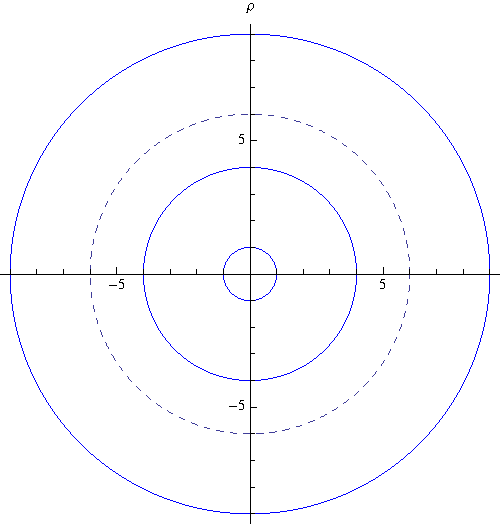
\includegraphics{Figures/cutoff}}
{
\caption[Yukawa orbits with cutoff]{A polar plot of the first three Bohr orbits along with a cutoff at $\lambda = 6$. Because the $n=3$ orbit lies outside the cutoff, it would not be allowed under \eqref{eq:naive}.}
\label{fig:cutoff}
}

This cutoff means that the relationship between $\rho$ and $n$ holds while $\rho < \lambda$, but breaks down after, limiting the number of bound states (figure \ref{fig:cutoff}). Any bound state allowed under \eqref{eq:rho-n} for which $\rho$ exceeds $\lambda$ will not exist. If we imagine increasing $\lambda$ gradually, a new bound state will be added whenever we pass through a point $\lambda = n^2$ (for some integer $n$). We call these points the critical values of lambda, notated $\lambda_{n}$, where $n = 1, 2, 3\ldots$ and corresponds to the number of bound states at that critical value. For the Coulomb potential with cutoff, then, $\lambda_{n} = n^2$.

\section{Application to Yukawa Potential}
To perform a more careful analysis of the potential, we look at the graph of its effective potential (figure \ref{fig:yveff}):
\eqn{
\tilde{V}_{\mathrm{eff}} = \frac{n^2}{\rho^2} - \frac{2}{\rho}e^{-\rho/\lambda}
\label{eq:yveff}
}
 
As before, we can see that bound states exist for some $n$ and $\rho$ where $V_{\mathrm{eff}}$ is less than 0, and these bound states have circular orbits at the minimum of $V_{\mathrm{eff}}$. However, there also appear to be bound states \emph{above} $E = 0$. Clasically, these are perfectly valid elliptical orbits. Quantum mechanically, a particle in one of these states can tunnel through and become a scattering state. This gives us two possible definitions for a critical value of $\lambda$.  The first is where the minimum of $V_{\mathrm{eff}}$ for some $n$ moves below zero -- that is, that value of lambda allows an additional stable bound state ($E < 0$). The other occurs where $V_{\mathrm{eff}}$ for some $n$ first starts to have a minimum at all, giving it a bound state with $E>0$. These two critical points are shown in figure \ref{fig:critpoints}

\begin{figure}[h]
\center{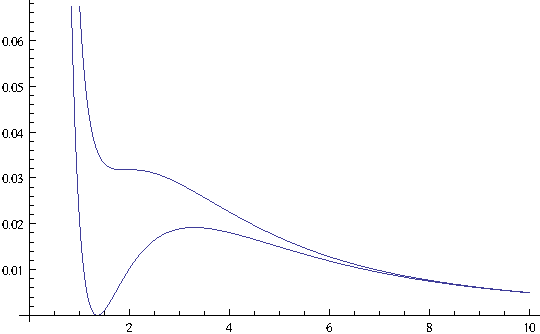
\includegraphics{Figures/criticalpoints}}
\caption[The two critical values of $\lambda$]{Two curves showing $V_{\mathrm{eff}}$ at the two critical values of $\lambda$ -- one where there are no more stable bound states, and one where there are no more bound states at all.}
\label{fig:critpoints}
\end{figure}

\begin{figure}[h]
\center{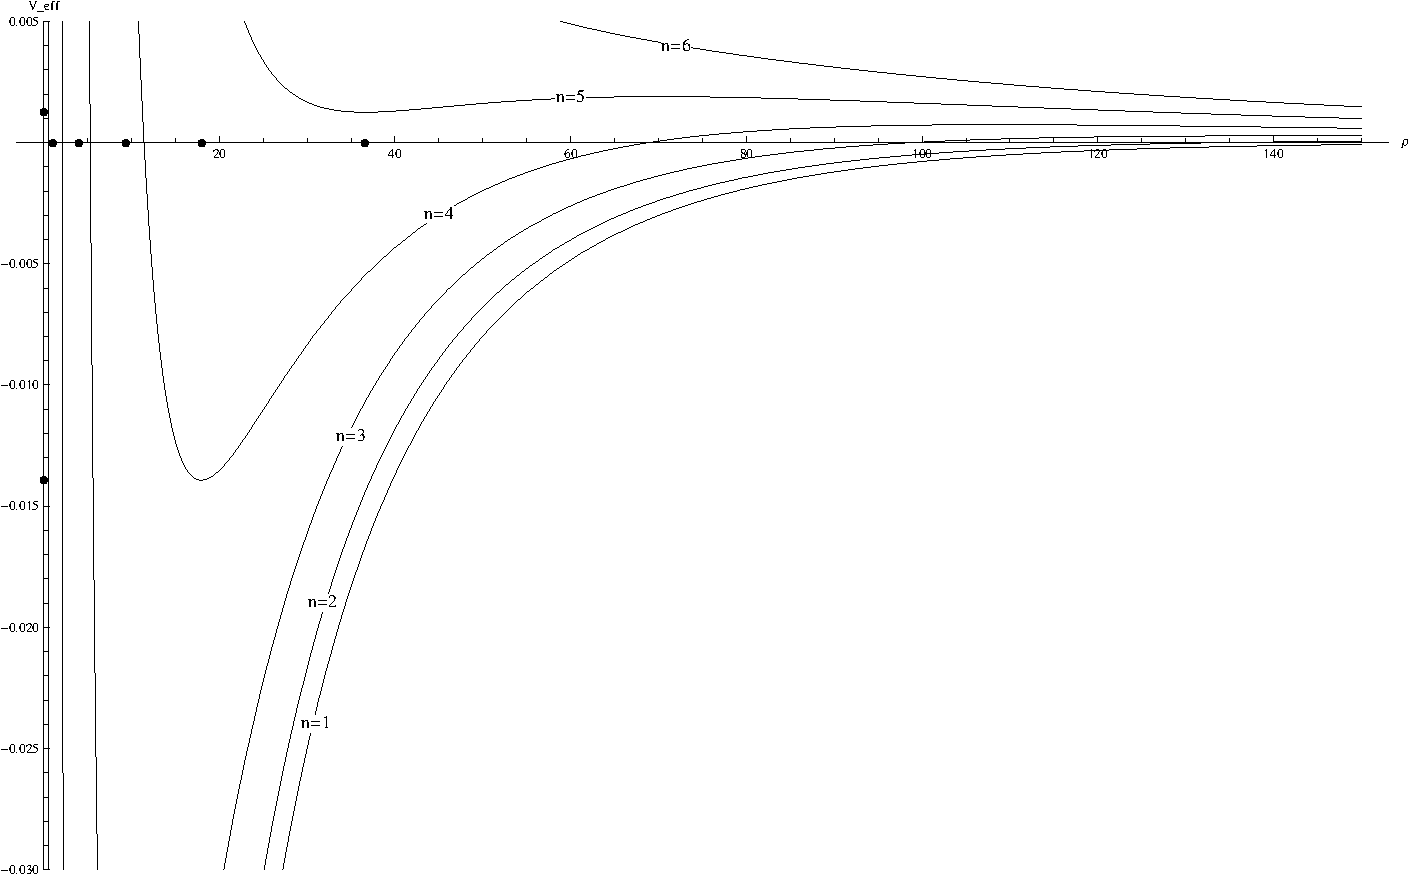
\includegraphics[width=\textwidth]{Figures/yukawa_Veff}}
\caption[The effective Yukawa potential]{The effective Yukawa potential. \eqref{eq:yveff} was plotted for $n = 1$ through $6$ with $\lambda = 32$. As with Coulomb, the curves get increasingly shallow as $n$ increases. The curves for $n = 1$ through $4$ all have a circular orbit with $E < 0$, that is, they have a stable bound state. The curve for $n = 5$ has a very slight minimum, but it does not go below $0$, meaning this corresponds to an unstable bound state. The $n = 6$ curve does not have a minimum at all. For all curves with a minimum, the approximate location of this minimum (obtained via Mathematica's NMinimize) has been plotted on the $\rho$ axis.}
\label{fig:yveff}
\end{figure}

\subsection{Stable bound states}
The first of these critical values occurs when the minimum of $V_{\mathrm{eff}}$ is 0. We again start by taking the derivative of \eqref{eq:yveff} and setting it to 0, obtaining
\begin{equation}
\frac{dV}{d\rho}\Big |_{\rho = \rho_0} =0 = -\frac{2n^2}{\rho_0^3} + \frac{2}{\rho_0^2}e^{-\rho_0/\lambda} + \frac{2}{\rho_0 \lambda} e^{-\rho_0/\lambda}
\label{vmin}
\end{equation}
where $\rho_0$ is the value of $\rho$ when $V_{\mathrm{eff}}$ is minimized. This equation holds for any $\lambda$ has no general solution, but we can find one for the specific case where $\lambda$ is some critical value $\lambda_n$ and $V_{\mathrm{eff}}(\rho_0) = 0$ by solving the equation
\begin{equation}
V_{\mathrm{eff}}(\rho_0)=0 = n^2 - 2\rho_0 e^{-\rho_0/\lambda_n} 
\end{equation}
for $n^2$
and plugging the result into \eqref{vmin}, obtaining
\begin{equation}
\rho_0 = \lambda_n \mbox{.}
\end{equation}
Plugging this back into the equation for $V_{\mathrm{eff}}(\rho_0)$, we find that
\begin{equation}
\lambda_n=\frac{e}{2}n^2=1.36 n^2
\label{eq:stable}
\end{equation}
which is pretty close to the behavior $\lambda_{n} = n^2$ from the cutoff Coulomb potential above. 

\subsection{Unstable bound states}

Having determined a formula for the $\lambda_n$s at which new bound states with $E < 0$ appear, we turn to the appearance of classically bound states with $E > 0$. A bound state exists when $V_{\mathrm{eff}}$ has a minimum. We found the $\rho_0$ where this minimum occurs in \eqref {vmin}, which we can rewrite as
\begin{equation}
n^2 = \left( \rho_0 + \frac{\rho_0^2}{\lambda} \right) e^{-\rho_0/\lambda}
\label{eq:unstablemins}
\end{equation}
The right side of this equation will have some maximum, which will be the last point for which the equation can be solved -- after that, the value of $n^2$ will always be greater than the right side. This is shown in figure \ref{fig:unstableveff}. For a given $n$, this gives $\lambda_n$.
\begin{figure}[h]
\centering
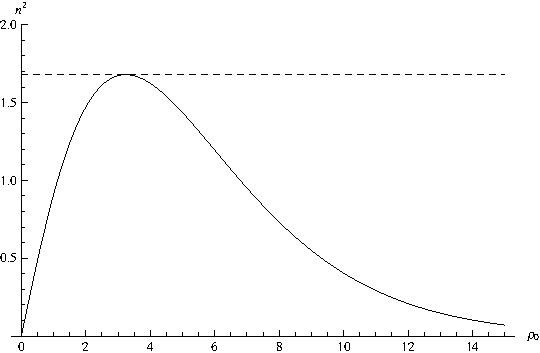
\includegraphics{Figures/unstableveff}
\caption[$n^2$ as a function of $\rho_0$]{This is a plot of \eqref{eq:unstablemins} with $\lambda = 2$, showing its maximum value. At this value of $\lambda$, the $n = 1$ bound state exists, because for $n = 1$ there is some $\rho_0$ that satisfies \eqref{eq:unstablemins}. This is not the case for the $n = 2$ bound state, so the $n = 2$ bound state does not exist. Increasing $\lambda$ scales the curve, increasing the number of bound states.}
\label{fig:unstableveff}
\end{figure}
To find this maximum, we differentiate with respect to $\rho_0$ and set the result 0, obtaining
\begin{equation}
0 = (1+2 \frac{\rho_0}{\lambda_n}) - \frac{1}{\lambda_n}(\rho_0 + \frac{\rho_0^2}{\lambda_n})\mbox{.} 
\end{equation}
This is a quadratic in $\rho_0$ and can be solved easily.
As $\rho_0$ is a real physical quantity that can't be negative, we can discard one solution, obtaining
\begin{equation}
\rho_0 = \frac{\lambda_n}{2}(1+\sqrt{5})\mbox{.}
\end{equation}
We can plug this in to \eqref{vmin} to find the relationship between $\lambda$ and $n$:
\begin{align}
n^2 &= \lambda_{n}(2 + \sqrt{5}) \\
\lambda_n &= 1.19 n^2
\label{eq:unstable}
\end{align}
\section{Summary}
Using the Bohr model to analyze the Yukawa potential yields three different expressions for the critical values $\lambda_n$: \eqref{eq:naive}, \eqref{eq:stable}, and \eqref{eq:unstable}. Each of these has the form 
\eqn{
\lambda_{n} = a n^2
}
where $a$ is some constant of order one. This suggests that when performing our numerics, we will find critical values of lambda that are proportional to the square of the number of bound states. 

We can apply this to deuterium and determine [fill in numbers here]

\clearpage %% starts a new page and stops trying to place floats such as tables and figures

\chapter{Numerical Methods and Spherically Symmetric Results}

In the previous chapter, we analytically obtained an estimate for the number of bound states allowed by the Yukawa potential given $\lambda$.  We now turn our attention to the Schr\"odinger Wave Equation in order to numerically determine the critical values of $\lambda$ at which a new bound state appears. In this chapter, we will focus on states with no angular momentum, which have spherically symmetric bound states.

\section{The Hamiltonian}

The Wave Equation can be written as
\eqn{
H \psi = E\psi
\label{eq:hamiltonian}
}
where $H$ is the Hamiltonian operator, $H =-\frac{\hbar^2}{2m}\nabla^2 +V$.  Because we are focusing on spherically symmetric bound states, we are only concerned about the $r$ component of the $\nabla$ operator. \eqref{eq:hamiltonian} then becomes
\eqn{
H = -\frac{\hbar^2}{2m} \left[\frac{1}{r^2}\frac{d}{dr}\left(r^2 \frac{d}{dr}\right)\right] - \frac{C}{r}e^{-r/l}\mbox{,}
}
plugging in the Yukawa potential for $V$.

Using the same nondimensionalizations as in last chapter, we rewrite this as 
\eqn{
H=\frac{C}{2\alpha}\tilde{H} = \frac{C}{2\alpha} \left[- \frac{1}{\rho^2}\frac{d}{d\rho}\left(\rho^2\frac{d}{d\rho}\right) - \frac{2}{\rho}e^{-\rho/\lambda}\right]\mbox{.}
\label{eq:hnondim}
}
The constant out front is the same one we pulled when we nondimensionalized the energy of the system, which allows us to restate \eqref{eq:hamiltonian} as
\eqn{
\tilde{H}\psi = \tilde{E}\psi\mbox{.}
}
To simplify, we can substitute \footnote{I should have a cite here.} $u(\rho)=\rho \phi(\rho)$ into the expression in \eqref{eq:hnondim}. This gives us a much neater Hamiltonian, and our differential equation is now
\eqn{
-\frac{d^2 u }{d \rho^2} - \frac{2}{\rho}e^{-\rho/\lambda}u = \tilde{E} u\mbox{.}
\label{eq:hamiltonianfinal}
}

\section{Numerics: The Finite Difference Method}
The finite difference method transforms a differential equation into a matrix problem. It does this by approximating the first and second derivatives of a function on a discrete grid of points $u(\rho_n) = u_n$ which are a distance $\Delta \rho$ apart. The grid runs from $u_1$ to some $u_N$. Using the concept of the derivative as the slope of the tangent line to some point, we can write
\eqn{
u'(\rho_n) = \frac{u(\rho_n + \Delta \rho) - u(\rho_n - \Delta \rho)}{2 \Delta \rho} - O(\Delta{\rho}^2)
\label{fdifference}
}
\eqn{
u''(\rho_n) = \frac{u(\rho_n + \Delta \rho) - 2 u(\rho_n) + u(\rho_n - \Delta \rho)}{\Delta \rho^2}-O(\Delta{\rho}^2) 
\label{f2difference}
}
We can rewrite this by applying \eqref{f2difference} to our differential equation in \eqref{eq:hamiltonianfinal}, obtaining
\eqn{
-u_{n-1}\frac{1}{\Delta \rho^2} - u_n\left(\frac{2} {\Delta \rho^2} -  \frac{2}{\rho_n}e^{-\rho_n/\lambda} \right) - u_{n-1}\frac{1}{\Delta \rho^2}  = E u_n\mbox{.}
\label{eq:hamiltonian-disc}
}
For the interior points, there are no concerns, but at the beginning we require a $u_0$ and at the end we need a $u_{N+1}$ in order to satisfy \eqref{eq:hamiltonian-disc}. For our problem, we set $u_0 = u(0)$  and $u_{N+1} = u(\infty)$. Because we cannot practically calculate anything infinitely far out, we define some $\rho_{\infty}$ and use $u(\rho_{\infty})$ as an approximation for $u(\infty)$. How good this is depends on how far out $\rho_{\infty}$ is set. We therefore require that $u(\rho_{\infty}) = 0$ in order to satisfy the condition that bound states go to 0 at infinity. 

We can now construct a Hamiltonian matrix using \eqref{eq:hamiltonian-disc}. The matrix will have entries on the off diagonal and diagonal and nowhere else:
\begin{equation*}H = \left(
\begin{array}{cccccc}
\frac{2} {\Delta \rho^2} -  \frac{2}{\rho_1}e^{-\rho_1/\lambda} & -\frac{1}{\Delta \rho^2} &  0 & 0 & 0 & 0 \\
-\frac{1}{\Delta \rho^2} & \frac{2} {\Delta \rho^2} -  \frac{2}{\rho_2}e^{-\rho_2/\lambda} &  -\frac{1}{\Delta \rho^2}  & 0 & 0 & 0 \\
0 &  -\frac{1}{\Delta \rho^2} & \frac{2} {\Delta \rho^2} -  \frac{2}{\rho_3}e^{-\rho_3/\lambda} &  -\frac{1}{\Delta \rho^2}  & 0 & 0 \\
 .&  . &.  &. & .& .  \\
 .& . & . & .& .&  . \\
0 & 0 &  0 & 0&  -\frac{1}{\Delta \rho^2} & \frac{2} {\Delta \rho^2} -  \frac{2}{\rho_N}e^{-\rho_N/\lambda}   \\
\end{array}
\right)
\end{equation*}
The eigenvectors of this matrix will be the wave functions $u(\rho_n)$, and the eigenvalues will be the energies of those wave functions. For the calculation of these eigenvalues and eigenvectors, we rely on Mathematica's built-in Eigenvalues[ ] command. Mathematica uses the sparseness of the array to optimize the calculation, speeding it up immensely. 

Using this, we can now see what our wave functions actually look like. For bound states where $n^2 << \lambda$, we find that the bound states look very similar to hydrogen (figure \ref{fig:hyd-yukawa}).
\begin{figure}[h]
\centering
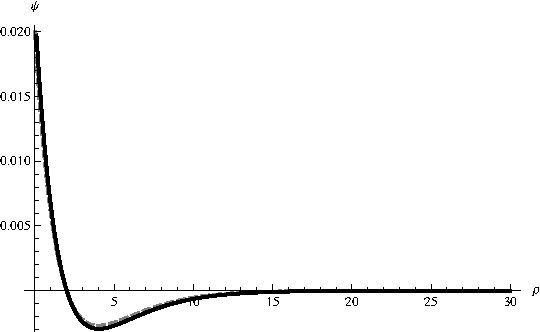
\includegraphics{Figures/n2hydyukawa}
\caption{The $n = 2$ bound states for the Yukawa potential and Coulomb potential. The Yukawa potential was calculated using my finite difference Hamiltonian with $\lambda = 20$ and  $\rho_{\infty} = 20*20 = 400$. The Coulomb wave function is the exact $n=2$ wave function, scaled by a constant to match the Yukawa function. The plot only extends out to $\rho = 30$ in order to see the earlier behavior; the function is remains 0 further out.}
\label{fig:hyd-yukawa}
\end{figure}
As $\lambda$ increases and more bound states are possible, the wave functions get more interesting, as in figure \ref{fig:largebound}.
\begin{figure}[h]
\centering
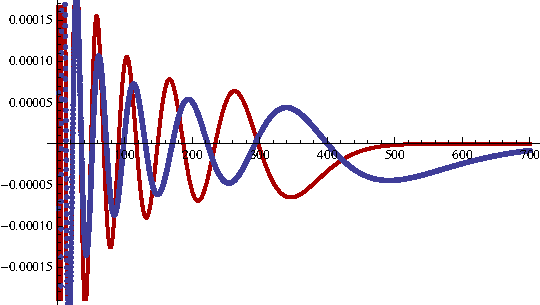
\includegraphics{Figures/hyukawa14}
\caption{The $n=14$ bound state at $\lambda = 200$. The $n=14$ Coulomb wave function is shown as well (scaled to match). At this value of $\lambda$, the $n=14$ state only recently became bound. While the Coulomb and Yukawa wavefunctions start out close together, the Coulomb wave function goes to zero faster and the wave functions diverge a bit towards the end. This plot shows the whole range where anything interesting is going on -- again, the function has gone to 0 and will stay there.}
\label{fig:largebound}
\end{figure}
\section{Finding Critical Values of Lambda}
Let us define a critical value of $\lambda$, $\lambda_n$ as the value of $\lambda$ where the Hamiltonian matrix gains a new negative eigenvalue. This is the point at which the function $u(\rho)$ gains a new bound state with energy less than zero. The subscript $n$ denotes the value of the principal quantun number, $n$, at this new eigenstate. This is the same type of thing as we used in chapter 1, updated for the quantum mechanical case.
At each value of lambda, we calculate the number of negative eigenvalues, and use rootfinding to look for a place where that number increases. For a further discussion of the exact methods used, see Appendix A.

We are looking for wave functions that behave like the ones in figure \ref{fig:scatt-to-bound}. In \subref{scatt12-5} the state is unambiguously scattering. While it does go to 0 at $\rho_{\infty}$, that's meaningless -- the way we set up our numerics requires it.
The function primarily looks like that of a free particle in a box of size $\rho_{\infty}$. 
 It doesn't level out much before it gets there, so it'll probably keep going right on through. In \subref{scatt12-9} it starts to level out, and in \subref{bound13-1} the state has become bound -- the function goes to zero before $\rho_{\infty}$ and stays there. Finally, in \subref{bound14} the state is clearly bound, going to 0 before $\rho_{\infty}$. 

\begin{figure}
\centering \subfloat[][$\lambda = 12.5$]{\label{scatt12-5}
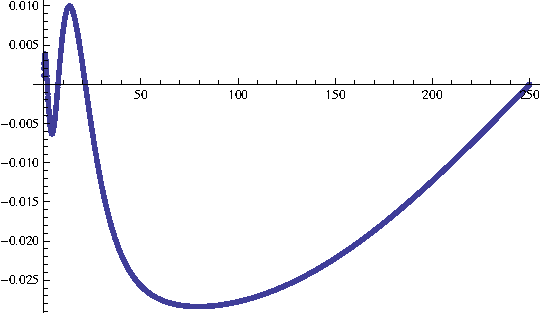
\includegraphics[width=0.5\textwidth]{Figures/12-5scatt}}
%\hspace{8pt}% 
\subfloat[][$\lambda = 12.9$]{\label{scatt12-9}
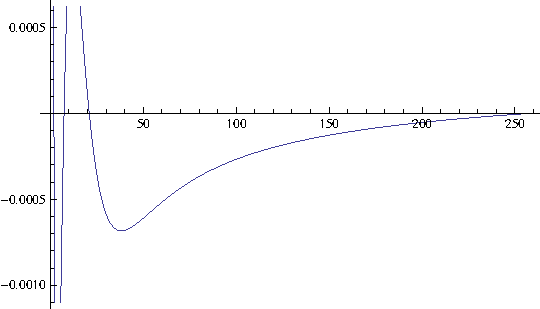
\includegraphics[width=0.5\textwidth]{Figures/12-9scatt}} \\ 
\subfloat[][$\lambda = 13.1$]{\label{bound13-1}
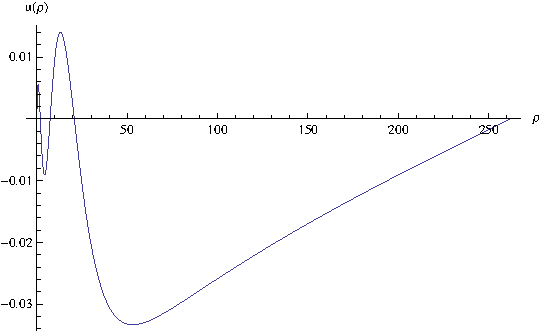
\includegraphics[width=0.5\textwidth]{Figures/13-1bound}}% \hspace{8pt}%
\subfloat[][$\lambda = 14.0$]{\label{bound14}%
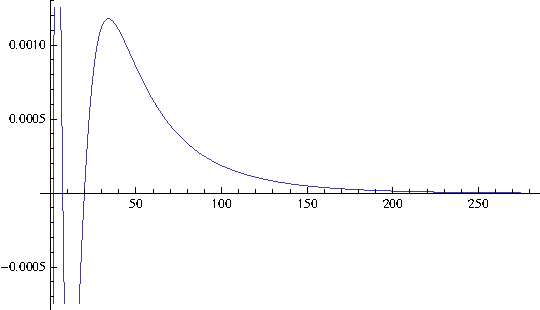
\includegraphics[width=0.5\textwidth]{Figures/14-bound}}
\caption[The progression of an eigenstate from scattering to bound]
{This figure shows the progression of the $n = 4$ eigenstate from scattering to bound. All wavefunctions were calculated with $\rho_{\infty} = 40 \lambda$ and $\Delta \rho = 0.1$.} 
\label{fig:scatt-to-bound}
\end{figure}

\section{Estimating errors}
In doing our numerical analyses, we would like to have a low $\Delta \rho$ -- after all, we expect the wave function to be interesting around 0. At the same time, we require $\rho_{\infty}$ to be large, because what separates bound states from scattering states is their behavior at infinity. This puts us in the frustrating numerical position of not really having anything we can skimp on to save computation time.

These, then, are our two primary sources of error. To determine the errors in each, we look at how much our calculated value for some $\lambda_{n}$ varies with changes in $\Delta \rho$ and $\rho_{\infty}$.  

To determine this, we looked at $\lambda_{4}$, chosen because it is relatively low, making the calculations quicker. We calculated the value of $\lambda_{4}$ at four different points: $\rho_{\infty} = 40*\lambda$ and $\Delta \rho = 0.1$, $\rho_{\infty} = 40*\lambda$ and $\Delta \rho = 0.05$, $\rho_{\infty} = 80*\lambda$ and $\Delta \rho = 0.1$, and $\rho_{\infty} = 80*\lambda$ and $\Delta \rho = 0.05$. The results of this are in table \ref{tab:errorchanges}. 
\begin{table}
\centering
\begin{tabular}{r|c|c|c|}
\multicolumn{1}{r}{}
 &  \multicolumn{1}{c}{$\rho_{\infty} = 40*\lambda$}
 & \multicolumn{1}{c}{$\rho_{\infty} = 80*\lambda$}
 & \multicolumn{1}{l}{} \\
\cline{2-4}
$\Delta \rho = 0.1$ & 12.8255 & 12.7543 & $\Delta \lambda_n = 0.0712$\\
\cline{2-4}
$\Delta \rho = 0.05$ & 12.8233 & 12.7521& $\Delta \lambda_n = 0.0712$ \\
\cline{2-4}
\multicolumn{1}{r}{}
 &  \multicolumn{1}{|c|}{$\Delta \lambda_n = 0.0022$}
 & \multicolumn{1}{c|}{$\Delta \lambda_n = 0.0022$}
 & \multicolumn{1}{l}{} \\
 \cline{2-3}
\end{tabular}
\caption{Errors in $\Delta \rho$ and $\rho_{\infty}$ for $\lambda_4$.}
\label{tab:errorchanges}
\end{table}
The changes in the calculated value for $\lambda_4$ from changes in $\Delta \rho$ and $\rho_{\infty}$ are independent of each other. We found that a change in $\rho_{\infty}$ produced a much bigger change in our calculated $\lambda_{n}$ than an equivalent change in $\Delta \rho$. Accordingly, we left $\Delta \rho$ fixed at 0.1 and only focused in errors in $\rho_{\infty}$. We decided to pin the value of $\rho_{\infty}$ to $\lambda$ in our calculations, which evened out the errors in different data points and allowed for more efficient calculations.

When we doubled $\rho_{\infty}$ a few more times, we found that the calculated values of $\lambda_{n}$ asymtotically decreased, approaching some true value. (figure \ref{fig:asymtote}). Because each point is closer to the true value than it is to the previous point, we can estimate the error by taking the distance between the two points and using that as error bars on the latter point.

\begin{figure}[h]
\centering
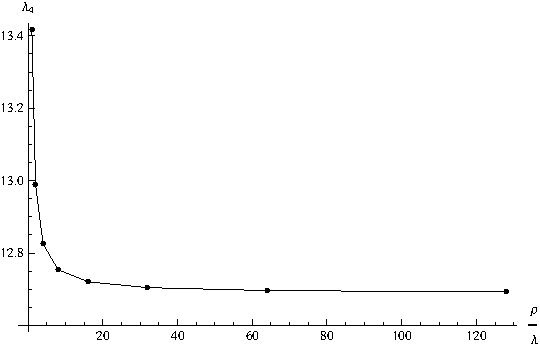
\includegraphics{Figures/asymtote}
\caption[Asymtotic behavior of $\lambda_{4} (\rho_{\infty})$]{The values of $\lambda_{4}$ as $\rho_{\infty}$ is repeatedly doubled, showing their asymtotic approach to some value. $\Delta \rho$ was held constant at 0.1. The $\rho_{\infty}$ values are given in terms of $\rho_{\infty}/\lambda$ in order to make the graph more clear.}
\label{fig:asymtote}
\end{figure} 

\section{Results and fit}
We ran our calculation for values of $\lambda$ between $0.5$ and $1000$, using a $\Delta \rho$ of 0.1 and a $\rho_{\infty}$ of $40$ and $80$ times $\lambda$ in order to capture errors in $\rho_{\infty}$ while keeping calculation times reasonable.

Our raw data, including error bars, is shown in figure \ref{fig:rawdata}. At a quick glance, it looks pretty quadratic -- just what we expected, but we needed to fit it to be sure.

\begin{figure}[h]
\centering
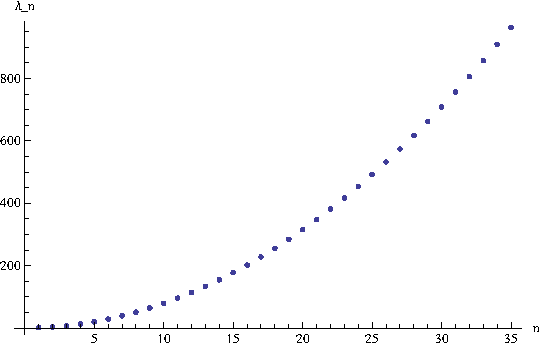
\includegraphics{Figures/rawdata}
\caption[Raw data for spherically symmetric $\lambda_n$s]{Raw data showing the locations of $\lambda_n$s with error bars from errors in $\rho_{\infty}$ Collected for $\lambda$ between 0.5 and 1000 with $\Delta \rho = 0.1$ and $\rho_{\infty} = 80*\lambda$.}
\label{fig:rawdata}
\end{figure}

Because we were looking for a relationship like $\lambda_n = a n^2$, we first tried a weighted linear fit to a log-log plot (figure \ref{fig:loglog}). Our fit was $\log(\lambda_n) = -0.22149 + 1.9947 \log(n)$. The coefficient of the $\log(n)$ term wasn't quite 2, and while the fit looked good, it was inaccurate, especially for low values of $n$. 
\begin{figure}[h]
\centering
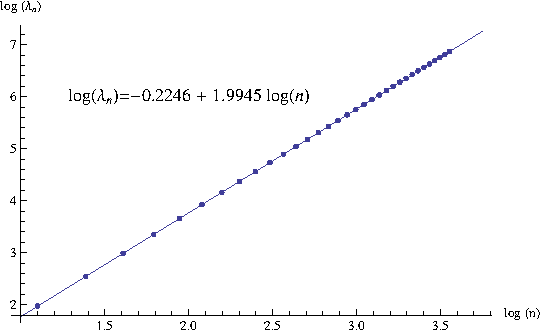
\includegraphics{Figures/loglog}
\caption[Log-log fit]{Linear fit to a log-log plot of the data from figure \ref{fig:rawdata}. Our fit was $\log(\lambda_n) = -0.22149 + 1.9947 \log(n)$.}
\label{fig:loglog}
\end{figure}

Based on this, we decided to try a fit to the equation $\lambda_n = a + b n + c n^2$ (figure \ref{fig:quadfit}). We found a general equation of $\lambda_n = 0.0578679 + 0.0517547 n + 0.785389 n^2$, which matched the data much better. Residuals for this fit were more random and did not conform to a pattern.
\begin{figure}[h]
\centering
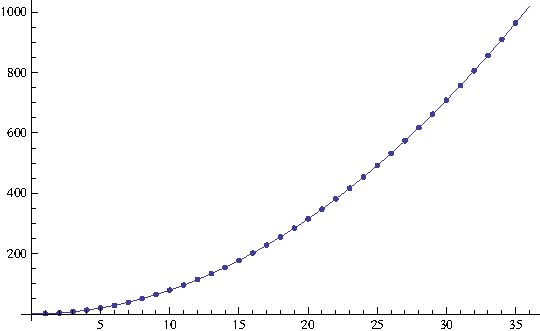
\includegraphics{Figures/quadfit}
\caption[Quadratic fit]{The data in figure \ref{fig:rawdata}, this time fit to a quadratic. The fit shown is $\lambda_n = 0.0578679 + 0.0517547 n + 0.785389 n^2$.}
\label{fig:quadfit}
\end{figure}

We computed the average error in $\lambda_n$ to check the goodness of fit. The calculated $\Delta \lambda_n$ was $0.0018454$ which is much lower than even our smallest $\Delta \lambda_n$ (0.0275888 for $\lambda_1$). This indicates that the fit is good and that the error estimation in the previous section likely overestimates the error in our numerical methods.

%\clearpage %% starts a new page and stops trying to place floats such as tables and figures

%
%
%\chapter*{Conclusion}
%         \addcontentsline{toc}{chapter}{Conclusion}
%	\chaptermark{Conclusion}
%	\markboth{Conclusion}{Conclusion}
%	\setcounter{chapter}{4}
%	\setcounter{section}{0}
%	
%
%If you feel it necessary to include an appendix, it goes here.
\appendix
\chapter{Numerical Methods}
To actually locate the critical values of lambda, we need to find the place where a new bound state appears. Numerically, this looks like a new negative eigenvalue in our list, which suggests we approach the problem with rootfinding. Our function has a ``zero'' whenever the number of negative eigenvalues increases.

Here it is in \emph{Mathematica} code:
\begin{Verbatim}[commandchars=\\\{\}, codes={\catcode`$=3}]
Critical[$\lambda$_, consts_] :=  Module[\{H, res, d$\rho$, $\rho$inf, nn\},
    d$\rho$ = consts[[1]];
    $\rho$inf = Round[consts[[2]]];
    nn = Round[$\rho$inf/d$\rho$];
    H = SparseArray[\{\{n_, n_\} -> 
        2./d$\rho$^2 - 2./(n*d$\rho$) $e$^(-n*d$\rho$/$\lambda$) + (
        l (l + 1))/(n*d$\rho$)^2, \{n_, m_\} /; Abs[n - m] == 1 -> -1./
        d$\rho$^2\}, \{nn, nn\}, 0.];
    res = Sort[Eigenvalues[H, -25]];
    Return[res]
  ]
\end{Verbatim}
This function takes a value of lambda and returns the some number of eigenvalues (here, 25)  of the hamiltonian which have the lowest absolute value. $nn$ is the matrix size, d$\rho$ is the step size, and $\rho$inf is numerical infinity for the problem.

The results of this calculation are extremely sensitive to $\rho$inf, and a larger $\rho$inf makes for less error. However, for larger values of $\rho$inf, more positive eigenvalues are found near 0, because the positive eigenvalues are in a continuous spectrum. As the grid becomes a better approximation of reality, more of these are picked up. This squeezes the negative eigenvalues (whose spectrum starts near -1) out, especially at higher values of $\lambda$. In order to ensure that there are *some* negative eigenvalues, we therefore pin $\rho$inf to some constant factor times $\lambda$. 

Increasing the number of negative eigenvalues found will also ensure we don't miss negative eigenvalues, but is very expensive. When searching for initial eigenvalues, we chose to get the 100 with the lowest absolute value in order to increase accuracy, but for the main calculation, 25 was fine.

The rootfinder actually used was a recursive bisection routine. In this rootfinder, we stopped recursing when the difference between the two endpoints was less than some $\delta$, instead of when the values of the function at the endpoints were within $\epsilon$. Because our function just looks at the number of negative eigenvalues, $f(\lambda_f) - f(\lambda_0)$ should always be equal to $1$ in a range with a zero and $\epsilon$ is meaningless. 

Again, in \emph{Mathematica} code:

\begin{Verbatim}[commandchars=\\\{\}, codes={\catcode`$=3}]
Bisect[F_, consts_, x0_, xf_, $\epsilon$_] := Module[\{mid, val, lnegs, vam, mnegs, vah\},
    mid = x0 + Abs[x0 - xf]/2;
    Print["Bisecting. Midpoint is " <> ToString[mid]]; (*progress indicator*)
    val = F[x0, consts];
    lnegs = CountNegs[val];
    vam = F[mid, consts];
    mnegs = CountNegs[vam];
    If[xf - x0 > $\epsilon$,
        If[lnegs < mnegs || (lnegs == mnegs && val[[1]] < vam[[1]]), 
            Return[Bisect[F, consts, x0, mid, $\epsilon$]];, 
            Return[Bisect[F, consts, mid, xf, $\epsilon$]]; 
     ];,
   vah = F[xf, consts];
   Return[{mid, lnegs, CountNegs[vah]}];
   ]
]
\end{Verbatim}

Again, when we bisect, we are looking at the number of negative eigenvalues as a function of lambda. In this routine, we assume multiple zeroes, and keep bisecting any range with a zero in it.

The complicated conditional for bisection is meant to deal with the problem of negative eigenvalues getting squeezed out by positive ones. Given a half of the input range, it bisects that half if either the number of negative eigenvalues increases (a regular zero), or the number of negative eigenvalues stays constant, but the value of the first negative eigenvalue jumps. This indicates that one negative eigenvalue was squeezed out, but another was added. In general, as $\lambda$ increases, the negative eigenvalues should decrease in value (coming closer and closer to the Coulomb energies). 

To find the ranges to bisect, we modify the rootfinder so it keeps bisecting as long as there is a zero in one of the ranges, and returns a list of points instead of just one. For efficiency's sake, this calculation is run at a low $\rho_{\infty}$, and a range is returned instead of a single point. That range can then be bisected more thoroughly in order to identify the most likely point. 

As is clear from the code, the function doing the actual work is just Mathematica's Eigenvalues[ ]. Because our Hamiltonian matrix only has entries on the diagonal and off-diagonals, we can define it as a SparseArray to speed up calculation. 

\section{Parallelization}

Finding a single $\lambda_{n}$ takes quite a bit of time -- it's expensive to find the eigenvalues of a large matrix, even such a sparse one as ours. We would like to study a wide range of $\lambda$s, and the computation begins to look prohibitively expensive.

This is where the cluster comes in. Mathematica has easy build in parallelization methods, and once we have ranges to bisect, each $\lambda_{n}$ calculation is independent from all the others. Distributing these calculations among multiple cores speeds the process up considerably, making this thesis possible.\footnote{I put this in because it felt like it should be in here, but have really no idea what to say.}

%      \chapter{The Second Appendix, for Fun}
%
%
%%This is where endnotes are supposed to go, if you have them.
%%I have no idea how endnotes work with LaTeX.
%
\backmatter % backmatter makes the index and bibliography appear properly in the t.o.c...
%
% Make my bibliography be called "Bibliography" and not "References" (or "Works Cited" or...):
%% \renewcommand{\bibname}{Works Cited}

 \bibliographystyle{plain}
%FIXME: should be apsrev.
  
% there are a variety of styles available; 
%% replace ``plainnat'' with the style of choice. You can refer to files in the bsts or APA 
%% subfolder, e.g. 
%% \bibliographystyle{APA/apa-good}  % or
%% \bibliographystyle{bsts/mla-good} 
%
%% if you're using bibtex, the next line forces every entry in the bibtex file to be included
%% in your bibliography, regardless of whether or not you've cited it in the thesis.
   \nocite{*}
   \bibliography{em_thesis}

% Finally, an index would go here... but it is also optional.
\end{document}
